\section{Design}
\label{sec:design}
We design a method for producing data placement configurations in NewSQL systems with tables partitioned and replicated in a manner to optimally colocate data with respect to a given query workload.  We look to previous database literature on automatically selecting materialized views for SQL databases. In many ways, selecting an optimal view to materialize is similar to selecting related table data to colocate as both involve finding and taking action on the most interesting table relationships with respect to a query workload.

\subsection{Estimating Colocation Benefits}
We first need to be able to quantify the benefit gained from colocating two tables.  For the view materialization problem in \cite{Yang:1997}, when considering a candidate view for materialization $V$, the query processing cost $C(Q,V)$ of a query workload $Q$ when using $V$ as the only view is examined.  With $S$ as the set of queries in $Q$, $q$ as a query in $S$, and $f_q$ as the frequency of $q$ in $Q$, this processing cost is intuitively:
\vspace*{-8pt}
\begin{equation}
C(Q,V) = \sum_{q \in S}f_qC(q,V)
\vspace*{-8pt}
\end{equation}
We reapply this equation to find the cost of a workload for a server when tables $s$ and $t$ are colocated in its memory as:
\begin{equation}
C(Q,s,t) = \sum_{q \in S}f_qC(q,s,t)
\vspace*{-5pt}
\end{equation}
This is essentially the cost of $Q$ when joins between $s$ and $t$ can be done locally on the server.  We also define $C(Q)$ to be the query processing cost of $Q$ for the server when it is never the case that the two tables required for any join are colocated in memory.  We define a distributed join to be a join where a server must fetch involved tables from different servers of the system for the join to be executed.  $C(Q)$ is thus the cost of executing $Q$ when all joins are distributed. The benefit of colocating $s$ and $t$ is thus:
\vspace*{-6pt}
\begin{equation}
Benefit(Q,s,t) = C(Q) - C(Q,s,t)
\vspace*{-8pt}
\end{equation}
We calculate $C(q,s,t)$, for any query $q$, based on our own heuristic cost model that estimates the number of row accesses required to perform the distributed joins of $q$. Only joins between tables from $\{s,t\}$ comes at no cost.  For each distributed join, we count the number of row accesses done to fetch both tables involved and perform the join.  For the purposes of our model, we assume that a server must even fetch $s$ or $t$ in a join with a table that is not from $\{s,t\}$.  We also assume the join is performed by scanning one table for each row of the other table.  For a query with distributed joins between any tables $A$, with $|A|_r$ rows, and $B$, with $|B|_r$ rows, and $s$ and $t$ colocated, we thus assign a cost of:
\vspace*{-4pt}
\begin{equation}
\label{eq:cost}
C(q,s,t) = \sum_{A\bowtie B\in q\mid A\notin \{s,t\} \lor B\notin\{s,t\}}|A|_r + |B|_r + |A|_r|B|_r
\vspace*{-4pt}
\end{equation}
\noindent This involves one access per row of both tables in order to fetch both tables and the product of the number of rows of both tables in order to execute the join.

\subsection{Partitioning}
We next decide how to optimally partition the data in a manner that avoids expensive distributed joins.  To do this, we define a weighted graph $G = (V,E)$ to represent the table relationships in the data model. Each node $v \in V$ represents a table in the data model. A directed edge $e = (u,v) \in E$ represents a foreign key relationship where $u$ is the "parent" table with the referenced key and $v$ is the "child" table with the foreign key. 
%The cost of an edge $c(e)$ is the cost to complete the query workload assuming that the two tables exists in the same server, or $C(Q,u,v)$.%
Let $DirectedBenefit(Q,s,t)$ be the same as $Benefit(Q,s,t)$ except that the benefit of colocation is only gained when $s$ is the parent and $t$ is the child of the join.  We then assign a weight to the edge $(u,v)$ equal to $DirectedBenefit(Q,u,v)$.  We refer the reader to Figure~\ref{fig:schema} for an example of what this graph looks like for the TPC-H schema.

Using $G$, we pick the $k$ best nodes (tables) to serve as partition "centers", meaning that we will pick the partitioning columns from these $k$ tables. To decide which tables are the $k$ best nodes to serve as partition centers, we define a benefit function $r_c$ which quantifies how useful a table would be if we picked a partitioning column from that table.
%Let $DirectedBenefit(Q,s,t)$ be the same as $Benefit(Q,s,t)$ except that the benefit of a join is only gained when $s$ is the parent and $t$ is the child.%
The function is defined as the sum of the weights of its outgoing edges added to the size of the table:
\vspace*{-8pt}
\begin{equation}
r_c(u) = \left( \sum_{e = (u,v)} DirectedBenefit(Q,u,v) \right) + |u|.
\vspace*{-7pt}
\end{equation}

The first part of the expression quantifies the benefit of colocating partitions of "child" tables with $u$, and the second part represents the fact that we generally want to partition larger tables. 

We pick the partition "centers" in an iterative process. We pick the node with the highest $r_c$ value and then remove this node and the nodes it was connected to in the graph. We then recompute $r_c$ for all the remaining nodes in the graph and iterate by picking the node with the highest value again until we have picked $k$ nodes.

Having picked these "centers", we then greedily assign other tables to partition and be colocated with them by assigning each table to the "center" for which its join on the partitioning column gives the most benefit.  We note that greedily assigning a table to a "center" may result in poor configurations in the case that the table has many important joins with tables that are not "centers".  We thus consider upgrading such tables to replicated tables in a later step.  If $S$ is the set of centers, a table $u$ is assigned to the center $A(u)$ as defined by:
\vspace*{-6pt}
\begin{equation}
A(u) = \max_{c \in S} \{DirectedBenefit(Q, c, u)\}
\vspace*{-6pt}
\end{equation}
Each "center" and its assigned tables make up what we call an entity group. An entity group is a unit for a set of tables that are all colocated and stored in the same server group.  If a table cannot be joined with any "center" on the partitioning key, it becomes a candidate for replication.

\begin{figure}
\centering
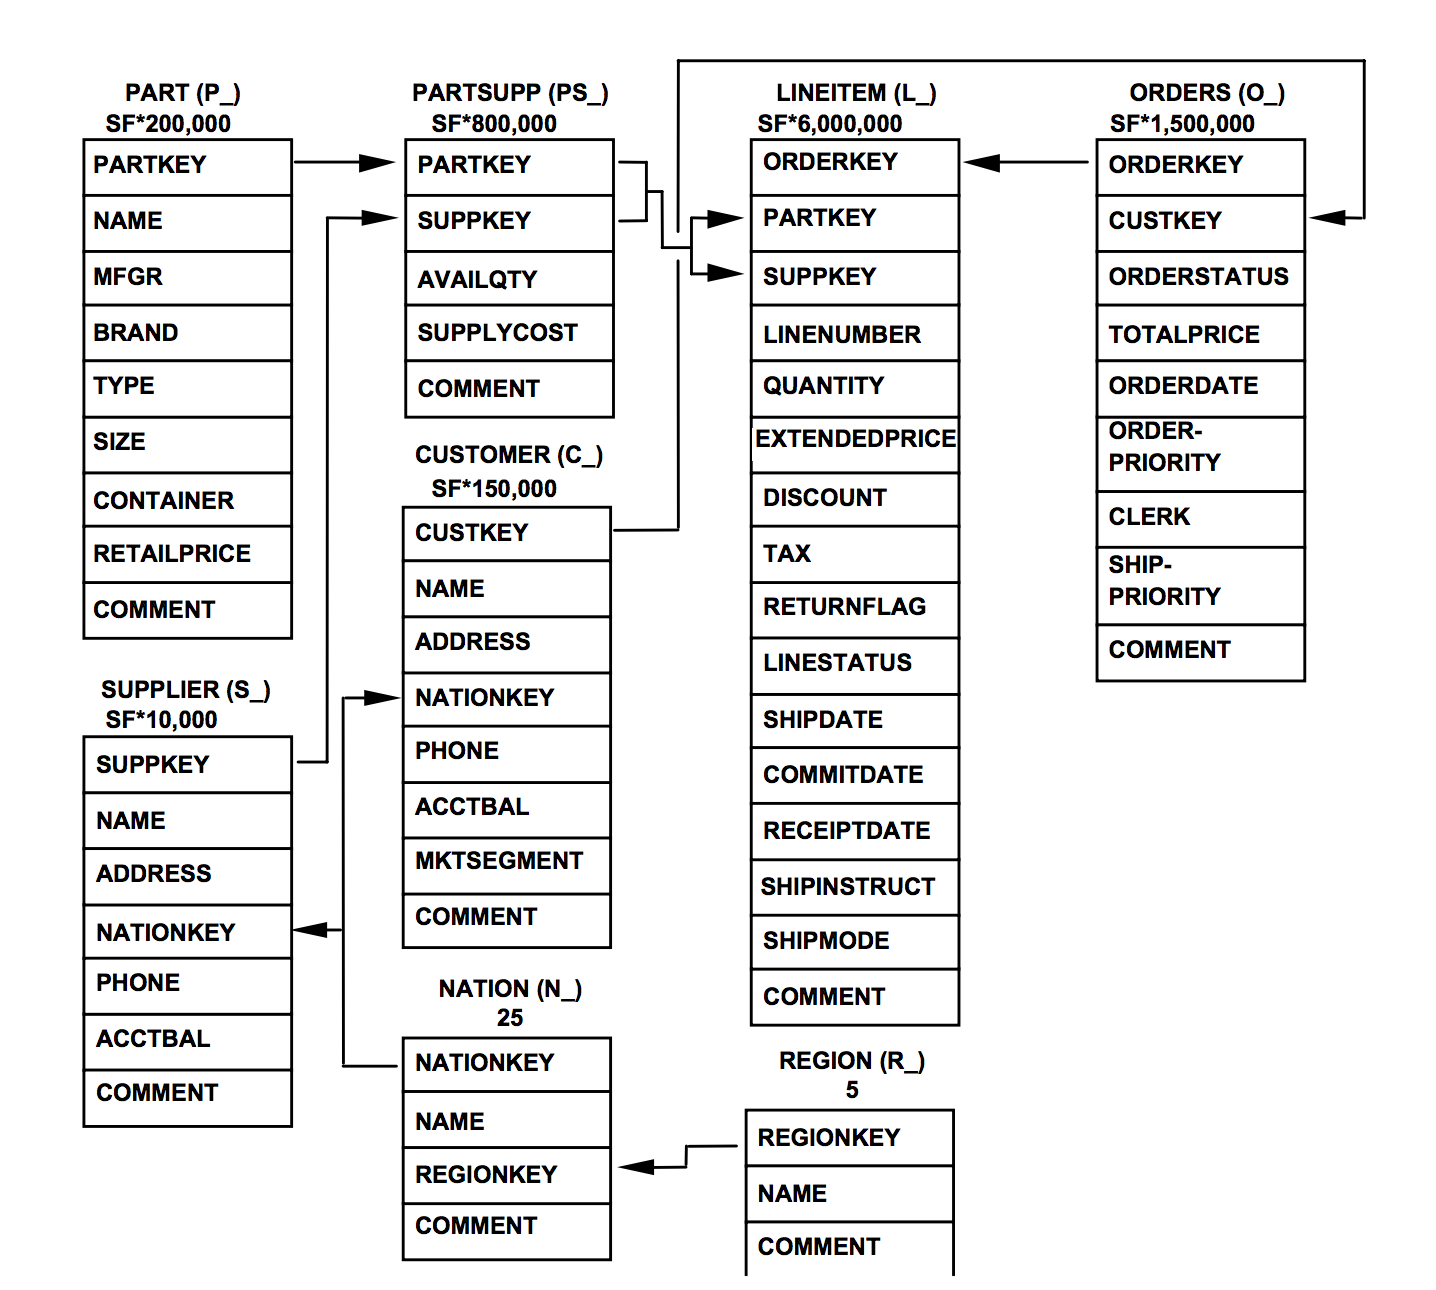
\includegraphics[scale=0.3]{TPC-H_DataModel.png}
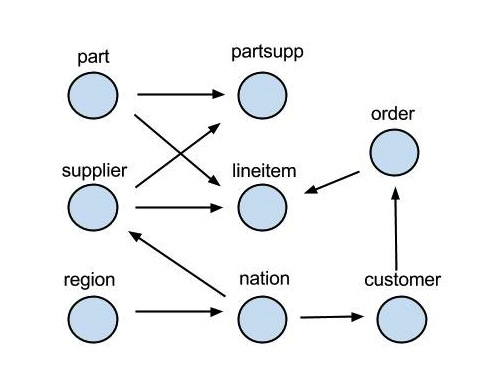
\includegraphics[scale=0.25]{ForeignJoinGraph.jpg}
\caption{\footnotesize{TPC-H Schema and corresponding graph produced without edge weights.}}
\label{fig:schema}
\end{figure}

\subsection{Replication}
In the next step, we decide which tables to pick to replicate in the system. The tables we consider for replication are those that are not partition centers.  Similar to with partitioning, we pick the $m$ best pairings of tables and entity groups to replicate into by defining a replication benefit function $r_r$, for each candidate table $u$ and entity group $E$. 

For each entity group $E$, given the average server memory size $\beta$, we can approximate the number of servers necessary to store $E$. Assuming $|P|$ is the sum of the sizes of the tables to be partitioned in $E$, we say this is 
\vspace*{-4pt}
\begin{equation}
\label{eq:numServers}
n = \lceil \frac{|P|}{\beta} \rceil
\vspace*{-4pt}
\end{equation}

Additionally, let $\phi(u)$ be the update rate of table $u$. The function $r_r$ quantifies the benefit of replicating table $u$ into the existing entity group $E$ as

\begin{equation}
\vspace*{-6pt}
r_r(u, E) = (\sum_{t \in E} Benefit(Q,t,u)) - |u| \cdot n - |u| \cdot \phi(u) \cdot n
\vspace*{-2pt}
\end{equation}

The first expression in the equation represents the benefit of colocating the replicated table in the entity group by enumerating the benefit gained by being able to do joins with $u$ and the tables in $E$ locally. The last two expressions in the equation represent the cost of colocating the replicated table by enumerating the cost to store the table at each server and the cost to send each update to the table synchronously to each server.  We rank the candidates by $r_r$ and then add the top $m$ replication candidates to the corresponding entity groups.  If a chosen replication candidate was partitioned and colocated with an entity "center" in the previous step, we override this decision and choose to replicate the table into one or more entity groups instead.

% This part can be cut based on how useful it is in the evaluation
\subsection{Server Assignment}
We now have entity groups containing an entity "center" and colocated partitions and replicated tables. In the last step, we consider assigning entity groups to a number of servers to form a server group.

Given the average server size, we can reuse Equation \ref{eq:numServers} to find the minimum number of servers needed to store an entity group $E$ while accounting for the space needed by the replicated tables in $E$. However, there is the question of how many servers to dedicate to $E$ beyond this minimum amount so that performance is optimal.

We do a cost-benefit analysis to determine how many servers to add beyond the minimum amount. Suppose the amount of servers assigned to $E$ is $n$; in the first iteration, $n$ is the minimum number of servers required. $m(n, E) = \frac{|P|}{n} + |R|$ gives the memory consumed by $E$ for a server when $E$ uses a server group of $n$ servers, $|P|$ is the sum of the sizes of the tables to be partitioned in $E$, and $|R|$ is the sum of the sizes of the replicated tables in $E$.  

With $\phi(R)$ as the average update rate of the tables in $R$, we repeatedly add a server to the group if 
\vspace*{-4pt}
{\small
\begin{equation}
b(n,E) = (m(n,E) - m(n+1,E)) - |R| - \phi(R) \cdot |R| > 0
\end{equation}
}
where $b(n,E)$ quantifies the point at which the cost of adding a server is greater than the benefit the extra server provides. The first part of the equation is the benefit of adding an additional server, as it represents the space savings a server gets through adding one more server to the group. The second part of the equation represents the cost of adding one more server due to additional replication and synchronous updates required.

We also accept a maximum number of servers parameter and stop adding servers to a server group before this parameter is exceeded.  Once a mapping of entity groups to server groups is produced, we leave it to the developer to map the server groups onto actual physical servers.

% \begin{figure}
% \centering
% \includegraphics[scale=0.50]{Flexible_Parallel.png}
% \caption{Flexible Parallel}
% \label{fig:flexible_parallel}
% \end{figure}
